\documentclass[french, 12pt]{article}
\usepackage[a4paper, top=2cm, bottom=2cm, left=2cm, right=2cm]{geometry}
\usepackage{fancyvrb}
\usepackage[T1]{fontenc}
\usepackage[french]{babel}
\usepackage{amsmath}  % Ajout du package amsmath

\usepackage{graphicx}
\usepackage{circuitikz}

\newcommand{\fct}[4]{%
  \begin{flalign*}  % Utilisation de l'environnement flalign
    #1: &\text{Entrée: } #2 \\
       &\text{Sortie: } #3 &\\
       &\text{Notes: } #4
  \end{flalign*}%
}

\begin{document}

TODO: Rendre l'affichage des fonctions plus beaux, j'ai créé une commande pour que ce soit facilement modifiable.
\section*{Fonctionnement du main}

Le fichier main.py s'occupe de définir le pc, les registres, les flags, et la ROM. À chaque cycle, il récupère toutes les anciennes valeurs grâce à des REG, fait appel aux différents modules et sélectionne la valeur souhaitée parmi les résultats renvoyés. Les différents modules appelés sont :
\begin{itemize}
    \item l'alu
    \item les décalages de bits
    \item les opérations sur la RAM
    \item les sauts dans le programme
\end{itemize}

Le circuit logique simplifié correspondant au main est donc :

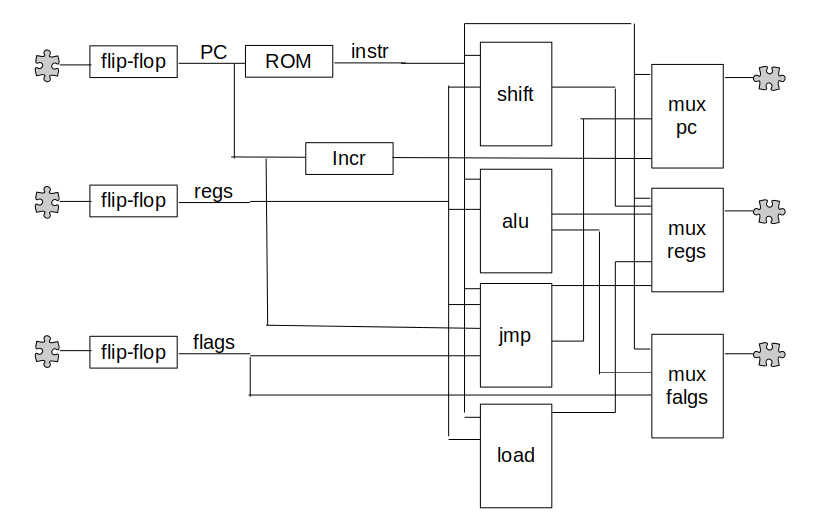
\includegraphics[width=17cm]{circuit_main.png}

\section*{L'ALU}

Le coeur du CPUlm. 

\subsection*{Fonctions auxiliaires}
Cette partie utilise les fonctions auxilliaires suivantes (toutes dans `alu.ply`):
\begin{itemize}
\item{
    \fct{big\_adder}{
        (b_i)_{i <= n}
    }{(s,c) \text{ correspondant à } \sum_{i=1}^n b_i}{}
}
\item{
    \fct{mul}{
        a \space b \text{ deux bus de même taille}
    }
    {(s,c) \text{ correspondant au produit}}
    {\text{Peut se désactiver avec le flag WITH\_MUL pour plus de performances.}}
}
\item{
    \fct{or\_n\_bits}{
        (b_i)_{i <= n}
    }
    {\vee_{i=1}^{n} b_i}
    {}
}
\item{
    \fct{div}
    {(a_i)_{i <= n} \text{ dividende,} (b_i)_{i <= n} \text{ diviseur}}
    {q \text{ quotient}}
    {}
}
\end{itemize}


\subsection*{Fonctionnement bref}

L'ALU prend deux arguments, l'instruction et les registres du cycle précédent.


L'instruction est passée selon cette syntaxe:\\


\begin{tabular}{|c|c|c|c|c|}
    \hline
    \multicolumn{1}{|c}{0:4} & \multicolumn{1}{c}{4:9} & \multicolumn{1}{c}{9:14} & \multicolumn{1}{c}{14:19} & \multicolumn{1}{c|}{19:24} \\
    \hline
    OP CODE & RD & RS1 & RS2 & ALUCODE \\
    \hline
  \end{tabular}\\


RD,RS1 et RS2 sont utilisés par les différentes instructions disponibles, les détails sont sur 
la documentation du processeur. Le code ALU est unique pour chaque instruction et est aussi disponible 
sur la doc du processeur. L'ALUCODE est utilisé dans un mux qui prend les différents calculs possibles en argument. 
rd (regsitre de destination) est modifié par un appel à update\_regs (cf tools.py). Enfin les flags sont mis à jour et la 
fonction renvoie les anciens flags et les flags mis à jour (c'est le main qui s'occupe de mettre à jour les regs).

\subsection*{Circuit de l'ALU}

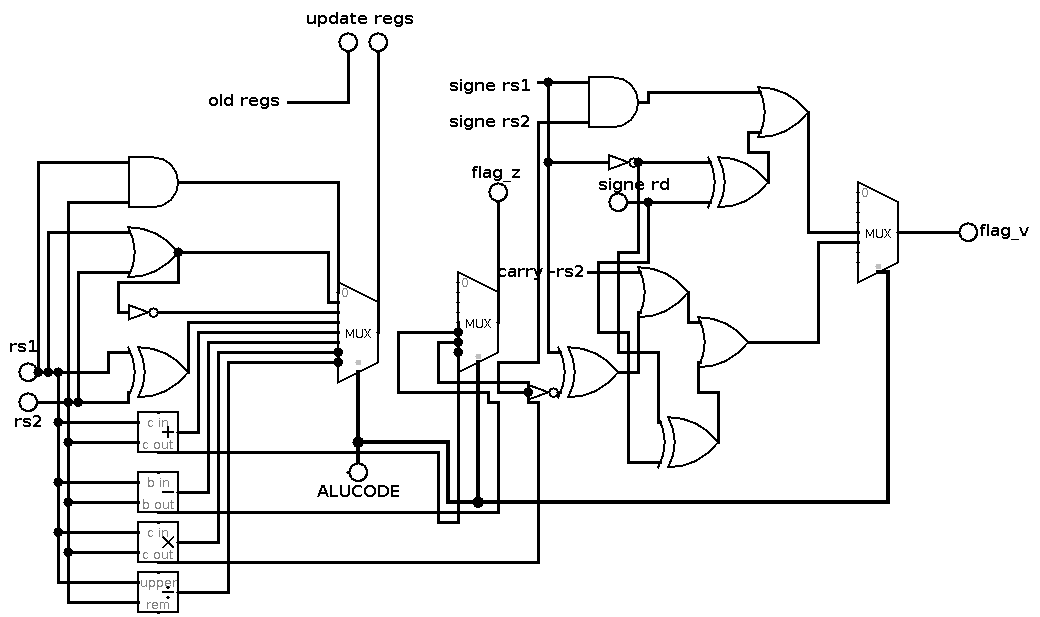
\includegraphics[width=17cm]{circuit_alu.png}

\section*{Les Jumps}

Todo

\section*{Les Shifts}

Todo

\end{document}

